\chapter{Technologies et outils utilisés}
\minitoc
\clearpage
\section{Introduction}
Comme cette application sera une application mobile, il est nécessaire que la performance soit la priorité lors du développement. C'est pourquoi on a choisi les technologies suivantes pour offrir une application rapide, performante, facile à utiliser.\\
\noindent Ses différentes technologies sont classifiées dans trois domaines principalement : Conception des interfaces graphiques, développement de l'application, et développement du back-end de l'application.\\
\section{Conception des interfaces utilisateur}
\subsection{Adobe Xd}
\vspace{1cm}
\begin{figure}[H]
    \centering
    
\includegraphics[width=0.25\textwidth]{xd_logo.png}
    \vspace{1cm}
    \captionsetup{justification=centering}

    \caption{Logo Adobe Xd}
    \label{fig:xd_logo}
\end{figure}
\textit{\textbf{Adobe Xd}} \cite{adobe_xd} est un outil de conception et modélisation des interfaces utilisateur des applications web et mobiles, développé par Adobe Inc.\\
\noindent Grâce aux outils fournis par Adobe Xd, la conception, l'amélioration et la rectification des interfaces graphiques et l'expérience de l'utilisateur de l'application sera plus facile, plus rapide et plus efficace.
\noindent Dans le cadre de ce projet, Adobe Xd a été utilisé pour la création des prototypes des interfaces graphiques, qui seront, par la suite, construits en application mobile à l'aide de Flutter.

Adobe XD n'est pas le seul outil disponible pour créer des prototypes, et concevoir les différentes interfaces utilisateur, Figma\cite{figma} est aussi un outil de conception et prototypage, développé par Figma Inc. qui a sorti sa première version en 2016 en tant qu'une application web.
\begin{table}[H]
    \begin{center}
        \begin{tabularx}{\textwidth}{| >{\centering\arraybackslash}X
                | >{\centering\arraybackslash}X
                | >{\centering\arraybackslash}X |}
            \hline
                                   & Adobe XD                                                       & Figma                                                                   \\
            \hline
            Plateformes            & Application Web.                                               & Application Desktop et Mobile.                                          \\
            \hline
            Système d'exploitation & MacOS, Linux, Windows.                                         & MacOS, Windows, iOS, Android.                                           \\
            \hline
            Collaboration          & Collaboration en temps réel.                                   & Collaboration en temps réel pour les projets sauvegardés dans le cloud. \\
            \hline
            Plugins                & Une bibliothèque riche en plugins créés pars les utilisateurs. & Une bibliothèque riche en plugins créés pars les utilisateurs.          \\
            \hline
        \end{tabularx}
        \captionsetup{justification=centering}
        \caption{Tableau comparatif: Adobe XD et Figma}
        \label{compare_adobexd_figme}
    \end{center}
\end{table}
Vu qu'on est en train de concevoir une application mobile, il est indisponible de tester les interfaces sous des appareils mobiles rapidement pour pouvoir les améliorer et détecter les défauts rapidement. C'est pourquoi on a choisi dans ce cas Adobe XD, grâce à sa plateforme cloud <<Adobe Creative Cloud>> qui permet de synchroniser les documents et les rendre disponibles sur toutes les plateformes disponibles.
\section{Développement de l'application mobile}
\subsection{Flutter}
\vspace{1cm}
\begin{figure}[H]
    \centering
    
\includegraphics[width=0.25\textwidth]{flutter.png}
    \vspace{1cm}
    \captionsetup{justification=centering}

    \caption{Logo Flutter}
    \label{fig:flutter_logo}
\end{figure}
\textit{\textbf{Flutter}} \cite{flutter} est un kit de développement (SDK) open-source créé par Google et publié en 2017.\\
\noindent Flutter permet de créer des applications mobiles (Android / iOS), web et même desktop (Windows / Linux / MacOS), avec une seule base de code en Dart, un langage de programmation développé aussi par Google. \\
\noindent Flutter présente plusieurs avantages qui permettent de créer des applications mobiles performantes et réduit aussi le coût et le temps de développement nécessaires, grâce au langage de programmation utilisé \textit{\textbf{Dart}} qui est très facile à maîtriser et qui offre plusieurs avantages, dont le plus important la fonctionnalité de <<\textit{\textbf{Hot Reload}}>> qui permet de recharger l'application et afficher les changements sur l'écran sans passer par la recompilation du code source.

Pour créer des applications mobiles crossplatform, Flutter n'est pas la seule technologie qui facilite le développement de ces applications. Il existe plusieurs autres alternatives dont on cite React Native\cite{react_native} qui permet aussi de créer une application mobile iOS et Android avec une seule base de code.
\begin{table}[H]
    \begin{center}
        \begin{tabularx}{\textwidth} {
                | >{\centering\arraybackslash}X
                | >{\centering\arraybackslash}X
                | >{\centering\arraybackslash}X |}
            \hline
                                     & Flutter                         & React Native                                \\
            \hline
            Créé par                 & Google.                         & Facebook.                                   \\
            \hline
            Langage de programmation & Dart.                           & Javascript.                                 \\
            \hline
            Hot Reload               & Oui.                            & Oui.                                        \\
            \hline
            Interfaces graphiques    & Utilise ses propres composants. & Utilise les composants natifs de chaque SE. \\
            \hline
            Taille de l'appplication & Plus petite que React Native    & Application volumineuse                     \\
            \hline
        \end{tabularx}
        \captionsetup{justification = centering}
        \caption{Tableau comparatif : Flutter et React Native}
        \label{compare_flutter_react_native}
    \end{center}
\end{table}
Comme le montre le tableau comparatif, Flutter a été le choix pour développer cette application grâce à sa capacité de créer des applications de petite taille qui sera toujours un avantage lors de son développement avec la liberté qu'il loffre lors de la création des composants de l'interface utilisateur qui permettra d'avoir des applications qui se rassemblent même s'ils sont sous différentes plateformes.


\section{Développement du serveur back-end}
\subsection{Express JS}
\vspace{1cm}
\begin{figure}[H]
    \centering
    
\includegraphics[width=0.25\textwidth]{express.png}
    \vspace{1cm}
    \captionsetup{justification=centering}
    \caption{Logo Express}
    \label{fig:express_logo}
\end{figure}
\textit{\textbf{Express JS}} \cite{expressjs} est un framework backend gratuit et open-source pour NodeJS. Créée par TJ Holowaychuk, la première version publique d'Express JS a été introduite au public en 2010.\\
Express JS est un framework minimaliste, très léger pour garantir une performance optimale et une exécution rapide. Ce framework est aussi très flexible, même s'il fournit que quelques fonctionnalités, grâce à \textit{\textbf{NPM}}, le gestionnaire de paquets de NodeJS, il peut être complété par plusieurs librairies disponibles.\\
\noindent Grâce à son minimalisme et facilité d'implémentation, ExpressJS est utilisé par plusieurs par nombreuses sociétés dans le monde, pour développer tout type d'applications, parmi ses sociétés il y a des géants de technologies tels que \textit{\textbf{IBM}}, \textit{\textbf{Uber}}, et plusieurs autres.


Spring Boot \cite{spring}, une extension du framework Spring, sorti en Avril 2014, est vu comme une alternative d' Express JS grâce à plusieurs avantages comme le montre le tableau suivant.
\begin{table}[H]
    \begin{center}
        \begin{tabularx}{\textwidth} {
                | >{\centering\arraybackslash}X
                | >{\centering\arraybackslash}X
                | >{\centering\arraybackslash}X |}
            \hline
                                    & ExpressJS        & Spring Boot                 \\
            \hline
            Utilisation de mémoire  & Faible.          & Élevée.                     \\
            \hline
            Multithreading          & Non              & Oui                         \\
            \hline
            Opérations Input/Output & Rapide           & Lent                        \\
            \hline
            Structure de projet     & Simple et léger. & Code complexe et modulaire. \\
            \hline
        \end{tabularx}
        \captionsetup{justification = centering}
        \caption{Tableau comparatif : ExpressJS et Spring Boot}
        \label{compare_spring_boot_expressjs}
    \end{center}
\end{table}
Comme la rapidité est l'un des objectifs de cette application, le temps de réponse à partir du serveur doit être minimal, ce qui offre ExpressJS grâce à NodeJS qui est très léger et qui peut être amélioré grâce aux dépendances de NPM.

\subsection{MongoDB}
\vspace{1cm}
\begin{figure}[H]
    \centering
    
\includegraphics[width=0.25\textwidth]{mongo.png}
    \vspace{1cm}
    \captionsetup{justification=centering}
    \caption{Logo MongoDB}
    \label{fig:mongo_logo}
\end{figure}
\textit{\textbf{MongoDB}} \cite{mongodb} , est un système de gestion de base de données NoSQL, orientée documents. Une base de données NoSQL est utilisée pour le stockage de volumes massifs de données, elle se distingue des des bases de données relationnelles par sa flexibilité et ses performances.\\
\noindent Le système MongoDB est développé par la société qui porte le même nom en 2007. Cette entreprise travaillait sur un système de cloud computing à données largement réparties.\\
\noindent Il est depuis devenu l'un des systèmes de gestion de base de données les plus utilisés, notamment pour des sites web très populaires tels que : \textit{\textbf{SourseForge.net}}, \textit{\textbf{eBay}} et \textit{\textbf{The New York Times}}.\\
\noindent Contrairement à une base de données relationnelle SQL traditionnelle, MongoDB ne repose pas sur des tableaux et des colonnes. Les données sont stockées sous forme de collections et de documents.
Les documents sont des paires de valeurs / clés servant d'unité de données de base. Les collections quant à elles contiennent des ensembles de documents et de fonctions. Elles sont l'équivalent des tableaux dans les bases de données relationnelles classiques.\\
\noindent On peut aussi utiliser MySQL\cite{mysql} qui est un Système de Gestion de Bases de Données créé par Oracle en 1995, qui est pour plusieurs, la solution idéale pour gérer leurs données.
\begin{table}[H]
    \begin{center}
        \begin{tabularx}{\textwidth} {
                | >{\centering\arraybackslash}X
                | >{\centering\arraybackslash}X
                | >{\centering\arraybackslash}X |}
            \hline
                                    & MongoDB                            & MySQL                           \\
            \hline
            Type de base de données & Base de données non relationnelle  & Base de données relationnelles  \\
            \hline
            Données structurées     & Non.                               & Oui                             \\
            \hline
            Design                  & Base sur le concept des documents. & Basé sur le concept des Tables. \\
            \hline
        \end{tabularx}
        \captionsetup{justification = centering}
        \caption{Tableau comparatif : MongoDB Code et MySQL}
        \label{compare_mongo_mysql}
    \end{center}
\end{table}


Vu que l'application SPN Cars n'utilise pas beacoup de jointures dans sa conception, et l'utilisation des données non structurés sera plus bénifique qu'utiliser des données structurés, le choix de MongoDB comme base de données el le choix le plus pertinent.

\subsection{JSON Web Token (JWT)}
\begin{figure}[H]
    \centering
    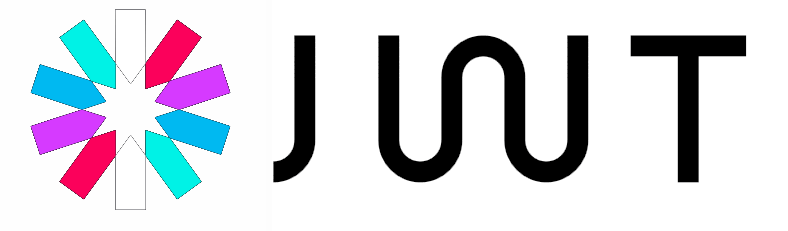
\includegraphics[width=0.25\textwidth]{jwt.png}
    \vspace{1cm}
    \captionsetup{justification=centering}
    \caption{Logo JWT}
    \label{fig:jwt_logo}
\end{figure}
\textbf{\textit{Josn Web Token}} ou tout simplement connu comme "JWT" est un standard créé en 2015, qui permet d'encapsuler des données dans des jetons et les échanger entre plusieurs parties en toute sécurité.

Un jeton est composé principalement de trois parties :
\begin{itemize}
    \item Un en-tête qui décrit le jeton en format JSON.
    \item Le contenu de ce jeton qui est également en format JSON.
    \item Une signature numérique.
\end{itemize}

\subsection{Firebase}
\vspace{1cm}
\begin{figure}[H]
    \centering
    
\includegraphics[width=0.25\textwidth]{firebase.png}
    \vspace{1cm}
    \captionsetup{justification=centering}

    \caption{Logo Firebase}
    \label{fig:firebase_logo}
\end{figure}
\textit{\textbf{Firebase}} \cite{firebase} est une plateforme créée en 2011, puis acquise et développée par Google en 2014. Firebase facilite la création de back-end à la fois scalable et performant.\\
\noindent L'objectif de firebase est d'offrir aux professionnels et aux particuliers un moyen d'éviter l'engagement dans un processus complexe de création et de maintenance d'une architecture serveur.\\
\noindent Firebase offre des API intuitives regroupées dans un SDK unique. Ces API permettent de gagner du temps et de réduire le nombre d'intégrations qu'on doit gérer dans l'application.\\
\noindent Firebase offre plusieurs services que tout le monde peut utiliser gratuitement grâce à sa politique <<pay as you go>> qui nécessite le paiement de ses services seulement si l'utilisation des ressources dépasse le quota du plan gratuit offert. Les services de Firebase les plus utilisés sont :
\begin{itemize}
    \item \textbf{Firestore}:\\ Une base de données NoSQL, bénéficiant d'un hébergement cloud et permettant le stockage et la synchronisation de données des utilisateurs.
    \item \textbf{Firebase Authentification}:\\ Un SDK prêt et facile à exploiter qui permet d'authentifier les utilisateurs en offrant plusieurs méthodes d'authentification tels que Google, Apple, Facebook, Email et mot de passe, numéro de téléphone et plusieurs d'autres méthodes pour assurer l'authentification de l'utilisateur.
    \item \textbf{Firebase Cloud Messaging}:\\ Permet de connecter plusieurs périphériques au serveur dans les meilleures conditions (fiabilité et économie de batterie). Ce service permet de recevoir et envoyer des notification sur les différentes plateformes (Web / iOS / Android). Avec Firebase Cloud Messaging, il est possible aussi d'assurer un service de messagerie instantanée entre les utilisateurs.
\end{itemize}
Dans ce projet, Firebase sera utilisé pour envoyer des notifications push vers les utilisateurs, mais ces service est aussi offert par OneSignal\cite{onesignal} qui est une solution qui offre les services d'envoi de notifications push, envoi de messages SMS et envoi d'emails.
\begin{table}[H]
    \begin{tabularx}{\textwidth} {
            | >{\centering\arraybackslash}X
            | >{\centering\arraybackslash}X
            | >{\centering\arraybackslash}X |}
        \hline
                                & Firebase                                                                          & OneSignal                                                                       \\
        \hline
        Open-Source             & Non                                                                               & Non                                                                             \\
        \hline
        Prix                    & Plan Gratuit trop limité, il est nécessaire d'acheter le pack "Growth" à \$9/mois & Gratuit, payer suivant la consommation après dépassement de seuil d'utilisation \\
        \hline
        Disponibilité           & 99.95\%                                                                           & 99.95\%                                                                         \\
        \hline
        Disponible pour Flutter & Oui                                                                               & Oui                                                                             \\
        \hline
    \end{tabularx}
    \captionsetup{justification=centering}
    \caption{Tableau comparatif: Firebase et OneSignal}
    \label{tab:compare_firebase_onesig}
\end{table}
Même si Firebase et OneSignl offrent les mêmes services, Firebase, grâce à sa flexibilité de calcul de frais de service en suivant le modèle <<Pay as you go>> réduit le coût de développement, ce qui rend Firebase le choix optimal pour envoyer des notifications vers les différents utilisateurs.
\subsection{Swagger}
\vspace{1cm}
\begin{figure}[H]
    \centering
    
\includegraphics[width=0.25\textwidth]{swagger.png}
    \vspace{1cm}
    \captionsetup{justification=centering}

    \caption{Logo Swagger}
    \label{fig:swagger_logo}
\end{figure}
\textit{\textbf{Swagger}} \cite{swagger} est un langage permettant de créer une description des API Restful à l'aide de JSON. A l'aide de ses outils Open-Source, Swagger permet de concevoir, créer et décrire des API REST.\\
\noindent Swagger a été créé en 2011 par Tony Tam, cofondateur du site de dictionnaires Wordnik, suite à un besoin d'automatisation de documentation de l'API qui est devenue de plus en plus frustrante. Juste après sa création, le projet Swagger est devenu open-source en septembre 2011.\\
\noindent Swagger est maintenant maintenu par la société \textit{\textbf{SmartBear Software}} qui, en novembre 2015, de créer une organisation appelée \textit{\textbf{OpenAPI initiative}} dont diverses entreprises tels que Google, IBM et Microsoft sont les membres fondateurs.\\
\section{Outils et logiciels}
\subsection{Visual Studio Code}
\begin{figure}[H]
    \centering
    
\includegraphics[width=0.25\textwidth]{vscode.png}
    \vspace{1cm}
    \captionsetup{justification=centering}
    \caption{Logo Visual Studio Code}
    \label{fig:vscode_logo}
\end{figure}
\textit{\textbf{Visual Studio Code}} \cite{vscode} est un éditeur de texte open-source développé par Microsoft \cite{microsoft} pour Windows MacOS et Linux en 2015. Riche en fonctionnalités tels que le support de déboguage, complétion intelligente du code, intégration de système de contrôle de version Git,et la capabilité d'installation d'extensions qui permettent d'améliorer l'expérience de l'utilisateur, Visual Studio Code est devenu l'un des premier choix pour plusieurs développeurs pour travailler sur leurs différents projets.

Pour développer des application mobiles avec Flutter, on peut utilisier Visual Studio Code ou Android Studio. Android Stduio qui est l'IDE utilisé pour développer des applications natives sous Android, qui est maintenant utilisé aussi pour développer les applications Flutter.
\begin{table}[H]
    \begin{center}
        \begin{tabularx}{\textwidth} {
                | >{\centering\arraybackslash}X
                | >{\centering\arraybackslash}X
                | >{\centering\arraybackslash}X |}
            \hline
                        & Visual Studio Code                                              & Android Studio                                                  \\
            \hline
            Taille      & Léger                                                           & Grande taille                                                   \\
            \hline
            Plugins     & Un store en ligne riche en plugins créés par les untilisateurs. & Un store en ligne riche en plugins créés par les untilisateurs. \\
            \hline
            Performance & Rapide et performant même sur une configuration faible.         & Nécessite une bonne configuration pour fonctionner fluidement   \\
            \hline
        \end{tabularx}
        \captionsetup{justification = centering}
        \caption{Tableau comparatif : Visual Studio Code et Android Studio}
        \label{compare_vscode_android_studio}
    \end{center}
\end{table}
Suite à cette comparaison, on a choisi Visual Studio Code grâce aux avantages qu'il offre tels que : La rapidité et fluidité d'usage est les extensions qui facilitent le développement des applications. Ces avantages permettront d'accélération du cycle de développement.
\subsection{Postman}
\begin{figure}[H]
    \centering
    
\includegraphics[width=0.25\textwidth]{postman.png}
    \vspace{1cm}
    \captionsetup{justification=centering}
    \caption{Logo Postman.}
    \label{fig:postman_logo}
\end{figure}
\textit{\textbf{Postman}} \cite{postman} est une plateforme permettant de concevoir, développer, et tester des API. Créé en 2012 comme une extension pour Google Chrome, Postman a gagné une grande popularité, qui lui a permis de migrer vers une application pour Windows MacOS, et Linux. Postman est maintenant le premier choix pour la plupart des développeurs, avec plus de 20 millions d'utilisateurs \cite{postman_users}.
Comme Postman, Insomnia REST Client\cite{insomnia} est aussi une plateforme qui permet d'effectuer des tâches similaires à Postman.
\begin{table}[H]
    \begin{tabularx}{\textwidth} {
            | >{\centering\arraybackslash}X
            | >{\centering\arraybackslash}X
            | >{\centering\arraybackslash}X |}
        \hline
                                              & Postman                                                            & Insomnia Rest Client            \\
        \hline
        Open-Source                           & Non                                                                & Oui                             \\
        \hline
        Gratuit                               & Oui                                                                & Oui                             \\
        \hline
        Documentation                         & Possibilité de générer automatiquement une documentation des APIs. & Ne génère pas de documentation. \\
        \hline
        Exécuter plusieurs reqûetes à la fois & Oui                                                                & Non                             \\
        \hline
    \end{tabularx}
    \captionsetup{justification=centering}
    \caption{Tableau comparatif : Postman et Insomnia REST Client}
    \label{tab:comparaison_postman_insomnia}
\end{table}
Avec la possibilité de générer automatiquement une documentation des APIs testés, et l'envoi de plusieurs requêtes à la fois, Postman est devenu le choix pour concevoir et tester les APIs qui seront utilisés par l'application SPN-Cars.
\subsection{Git}
\vspace{1cm}
\begin{figure}[H]
    \centering
    
\includegraphics[width=0.25\textwidth]{git.png}
    \vspace{1cm}
    \captionsetup{justification=centering}

    \caption{Logo Git.}
    \label{fig:git_logo}
\end{figure}
\textit{\textbf{Git}} \cite{git} est un système de contrôle de version open-source créé en 2005 par \textit{\textbf{Linus Torvalds}}, le créateur du noyau du système d'exploitation Linux.\\
\noindent Git permet de gérer les ajouts et changements apportés au code source de manière tracée. Ainsi, si une erreur est commise, les développeurs peuvent revenir en arrière et comparer les versions antérieures du code, ce qui leur permet de corriger l'erreur tout en minimisant les perturbations pour tous les membres de l'équipe.
\section{Conclusion}
Suite à l'étape de conception vue dans le chapitre précédent, on a présenté les outils et technologies qui ont été choisis pour le développement de ce projet.\\
\noindent Chaque outil et technologie a été choisi suite à une étude du besoin et une comparaison avec les différents compétiteurs disponibles.\\
Une fois ces technologies choisies, on passera vers la dernière étape qui est la réalisation de cette application qui sera présentée dans le chapitre suivant.